\documentclass[]{book}

%These tell TeX which packages to use.
\usepackage{array,epsfig}
\usepackage{amsmath}
\usepackage{amsfonts}
\usepackage{amssymb}
\usepackage{amsxtra}
\usepackage{amsthm}
\usepackage{mathrsfs}
\usepackage{color}
\usepackage{graphicx}
\usepackage{float}

%Algorithm packages
\usepackage{algorithm}  
\usepackage{algpseudocode}  
\usepackage{amsmath}  
\renewcommand{\algorithmicrequire}{\textbf{Input:}}  % Use Input in the format of Algorithm  
\renewcommand{\algorithmicensure}{\textbf{Output:}} % Use Output in the format of Algorithm  
%Here I define some theorem styles and shortcut commands for symbols I use often
\theoremstyle{definition}
\newtheorem{defn}{Definition}
\newtheorem{thm}{Theorem}
\newtheorem{cor}{Corollary}
\newtheorem*{rmk}{Remark}
\newtheorem{lem}{Lemma}
\newtheorem*{joke}{Joke}
\newtheorem{ex}{Example}
\newtheorem*{soln}{Solution}
\newtheorem{prop}{Proposition}

\newcommand{\lra}{\longrightarrow}
\newcommand{\ra}{\rightarrow}
\newcommand{\surj}{\twoheadrightarrow}
\newcommand{\graph}{\mathrm{graph}}
\newcommand{\bb}[1]{\mathbb{#1}}
\newcommand{\Z}{\bb{Z}}
\newcommand{\Q}{\bb{Q}}
\newcommand{\R}{\bb{R}}
\newcommand{\C}{\bb{C}}
\newcommand{\N}{\bb{N}}
\newcommand{\M}{\mathbf{M}}
\newcommand{\m}{\mathbf{m}}
\newcommand{\MM}{\mathscr{M}}
\newcommand{\HH}{\mathscr{H}}
\newcommand{\Om}{\Omega}
\newcommand{\Ho}{\in\HH(\Om)}
\newcommand{\bd}{\partial}
\newcommand{\del}{\partial}
\newcommand{\bardel}{\overline\partial}
\newcommand{\textdf}[1]{\textbf{\textsf{#1}}\index{#1}}
\newcommand{\img}{\mathrm{img}}
\newcommand{\ip}[2]{\left\langle{#1},{#2}\right\rangle}
\newcommand{\inter}[1]{\mathrm{int}{#1}}
\newcommand{\exter}[1]{\mathrm{ext}{#1}}
\newcommand{\cl}[1]{\mathrm{cl}{#1}}
\newcommand{\ds}{\displaystyle}
\newcommand{\vol}{\mathrm{vol}}
\newcommand{\cnt}{\mathrm{ct}}
\newcommand{\osc}{\mathrm{osc}}
\newcommand{\LL}{\mathbf{L}}
\newcommand{\UU}{\mathbf{U}}
\newcommand{\support}{\mathrm{support}}
\newcommand{\AND}{\;\wedge\;}
\newcommand{\OR}{\;\vee\;}
\newcommand{\Oset}{\varnothing}
\newcommand{\st}{\ni}
\newcommand{\wh}{\widehat}

%Pagination stuff.
\setlength{\topmargin}{-.3 in}
\setlength{\oddsidemargin}{0in}
\setlength{\evensidemargin}{0in}
\setlength{\textheight}{9.in}
\setlength{\textwidth}{6.5in}
\pagestyle{empty}



\begin{document}


\begin{center}
{\Large COMP 540 \hspace{0.5cm} HW 4}\\
\textbf{Peiguang Wang, Xinran Zhou}\\ %You should put your name here
Due: 3/5/2018 %You should write the date here.
\end{center}

\vspace{0.2 cm}


\subsection*{1: Intuitions about support vector machines }

%% Problem 1
\begin{enumerate}
	\item We typically frame an SVM problem as trying to maximize the margin. Explain intuitively why a bigger margin will result in a model that will generalize better, or perform better in practice.
	\begin{soln}
		Because with larger margin, we have more confidence to our result. That is, we have more confidence to classify a given sample to its class. The points that are most difficult to classify, which lies close to the decision boundary, can be classify using the boundary or hyperplane found by maximum margin.
		Also, we can reduce overfitting with bigger margin.
	\end{soln}
	\item Will moving points which are not support vectors further away from the decision boundary effect the SVM’s hinge loss?
	\begin{soln}
		hinge loss function
		$$hinge loss = max(0,1-y^{(i)}(\theta^T x^{(i)} + \theta_0))$$
		No. For those points that lie on both sides, the right hand of the max function is already negative. And that will stay negative as moving them further away from the decision boundary. So the hinge loss will always be zero. The loss function and decision boundary are only determined by the support vectors.
	\end{soln}
\end{enumerate}
\subsection*{2: Fitting an SVM classifier by hand}
\begin{enumerate}
	\item Write down a vector that is parallel to the optimal vector $\theta$.
	\begin{soln}
	After mapping the points to the 3-D using feature vector $\phi(x)$, new data $D^{'}$ is
	$$D^{'} = \{([1,0,0],-1),([1,2,2],+1)\}$$
	since there are only two points, the vector	$\theta$ is parallel to the direction of two connected points, so 
	$$\theta = (0,2,2)$$
	
	\end{soln}
	\item What is the value of the margin that is achieved by this $\theta$?
	\begin{soln}
		Because we only two sample points, so the margin achieved by this $\theta$ is equal to the distance of two points. That is $2\sqrt{2}$
	\end{soln}
	\item Solve for the θ.
	\begin{soln}
		From the previous part, we know that the margin is equal to $2\sqrt{2}$. Therefore,
		$$\frac{2}{||\theta||} = 2\sqrt{2}$$
		subject to $\theta = k(0,2,2)$ 
		so we can solve the equation and get $\theta = (0,\frac{1}{2},\frac{1}{2})$
		
	\end{soln}
	\item Solve for the intercept $\theta_0$ using your value for $\theta$ and the inequalities above.
	\begin{soln}
		We already know that for dataset $D^{'}$.
		$$y^{(1)}(\theta^T x{(1)}+ \theta_0)\geq1$$
		$$y^{(2)}(\theta^T x{(2)}+ \theta_0)\geq1$$
		using the $\theta$ that we got from the previous part, we can finally get
		$$ -1\leq\theta_0\leq -1$$
		so $\theta_0 = -1$
		
	\end{soln}
	\item Write down the equation for the decision boundary in terms of $\theta$, $\theta_0$ and x.
	\begin{soln}
		The decision boundary should be $\theta^T X + \theta_0 = 0$
		where $X = \varPhi(x) = (1,\sqrt{2}x,x^2)$.
		So the decision boundary is 
		$$\frac{\sqrt{2}}{2} x + \frac{1}{2} x^2 -1 = 0$$
	\end{soln}
	
\end{enumerate}
\subsection*{Problem 3: Support vector machines for binary classification - Part 1}
\begin{enumerate}
	\item The hinge loss function and gradient.
	\begin{soln}
	The implementation of  the hinge loss cost function and its gradient for support vector machines.
	
	The cost $J$ and the gradient of the loss function with respect to an all-zeros θ vector are computed.
	\begin{figure}[H]
		\centering
		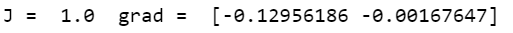
\includegraphics[width=8cm]{j.png}
		\caption{the result of the hinge loss and gradient}
		\label{fig:1}
	\end{figure}
	\end{soln}
	\item Example dataset 1: impact of varying C.
	\begin{soln}
		The C parameter is a positive value that controls the penalty for misclassified training examples. Large C will tell the SVM model try to classify all the samples correctly. Here I change the value of C on the decision boundary to see the different decision boundary.
		\begin{figure}[H]
			\centering
			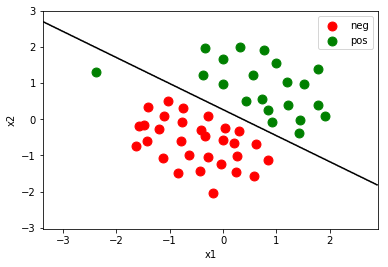
\includegraphics[width=8cm]{c1.png}
			\caption{SVM decision boundary with C = 1 for Example dataset 1}
			\label{fig:2}
		\end{figure}
		\begin{figure}[H]
			\centering
			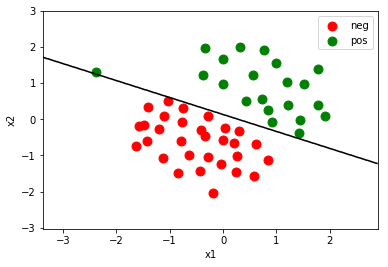
\includegraphics[width=8cm]{c100.png}
			\caption{SVM decision boundary with C = 100 for Example dataset 1}
			\label{fig:3}
		\end{figure}
		When C = 1, we can see that the boundary misclass an example. It's because of the weak regulation. As C increase, the penalty for misclassification will be larger, resulting less misclassified points.
	\end{soln}
	\item Gaussian kernel
	\begin{soln}
		Implement the Gaussian kernel function and test our implementation.
		\begin{figure}[H]
			\centering
			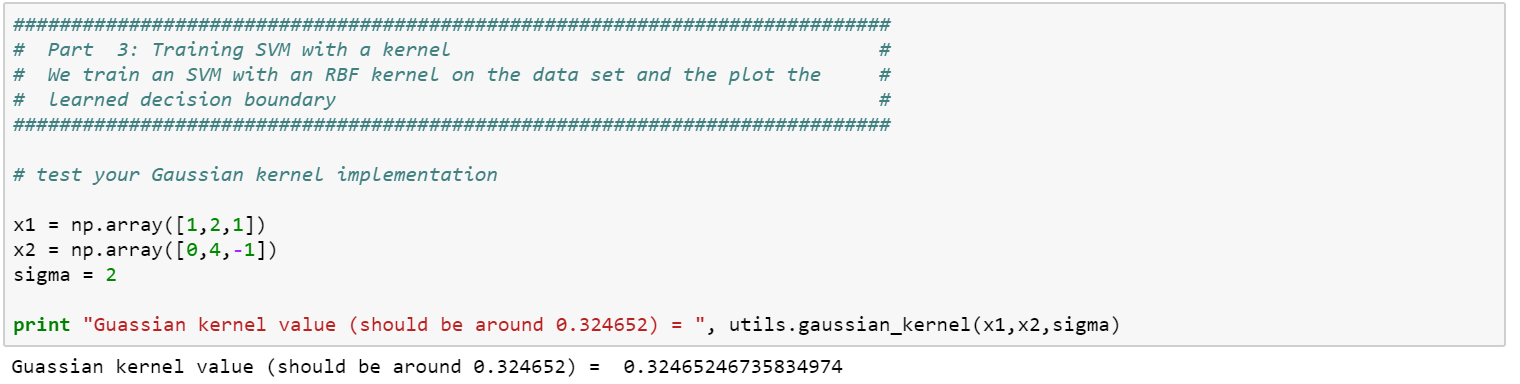
\includegraphics[width=12cm]{gaussian.png}
			\caption{the Guassian kernel value }
			\label{fig:4}
		\end{figure}
	\end{soln}
	\item Example dataset 2: learning non-linear boundaries.
	\begin{figure}[H]
		\centering
		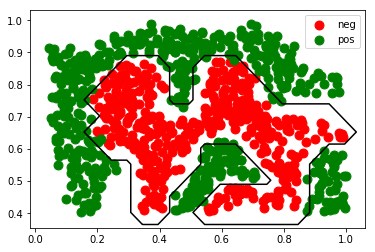
\includegraphics[width=8cm]{dataSet2.png}
		\caption{SVM gaussian kernel decision boundary for Example dataset 2, C = 1 and $\sigma$ = 0:02 }
		\label{fig:5}
	\end{figure}
	\item Example dataset 3: selecting hyper parameters for SVMs.
	\begin{soln}
		Selecting the best C and $\sigma$ parameter using cross-validation. The best C and $\sigma$ is shown in figure 6
		\begin{figure}[H]
			\centering
			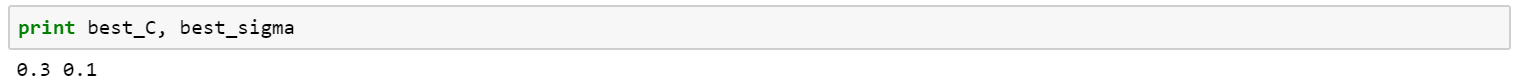
\includegraphics[width=8cm]{bestc.png}
			\caption{selection the best C and $\sigma$ }
			\label{fig:6}
		\end{figure}
		The corresponding decision boundary given the best C and $\sigma$ is shown in figure 7
		\begin{figure}[H]
			\centering
			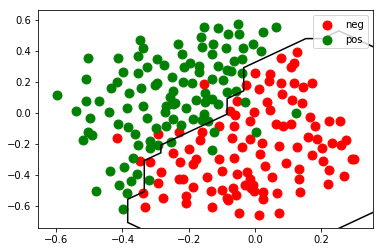
\includegraphics[width=8cm]{seHyperparameters.png}
			\caption{SVM Gaussian kernel decision boundary for Example dataset 3 with the best hyper parameters.}
			\label{fig:7}
		\end{figure}
	\end{soln}
\end{enumerate}
\subsection*{Problem 3: Support vector machines for binary classification - Part 2 Spam Classification }

Because the data X we got is one-hot encoded, which consist only 0 and 1. So we think there is no need to use Gaussian kernel. And X is near 0, so there is no need to scale either. Using cross-validation to select the hyperparameters, the best accuracy is reached by setting C = 1, learning rate = 0.3, and iteration number is 10000.
Here are some results, more detailed results can be found in the .HTML file.

\begin{figure}[H]
	\centering
	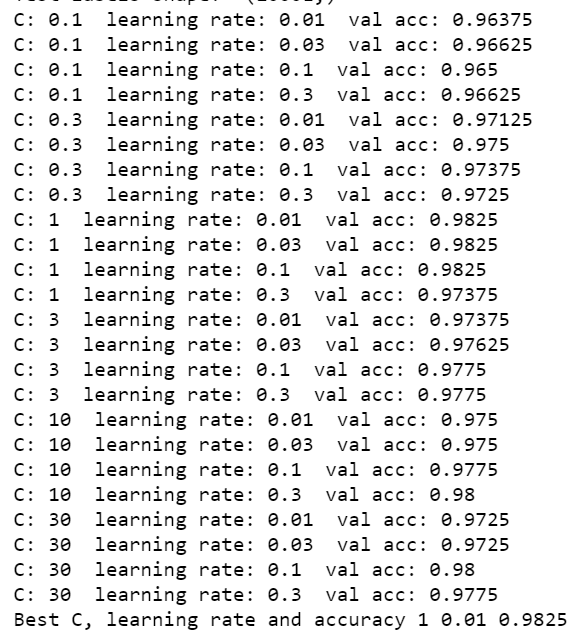
\includegraphics[width=8cm]{xuan.png}
	\caption{selecting the best hyperparameters}
	\label{fig:8}
\end{figure}
\begin{figure}[H]
	\centering
	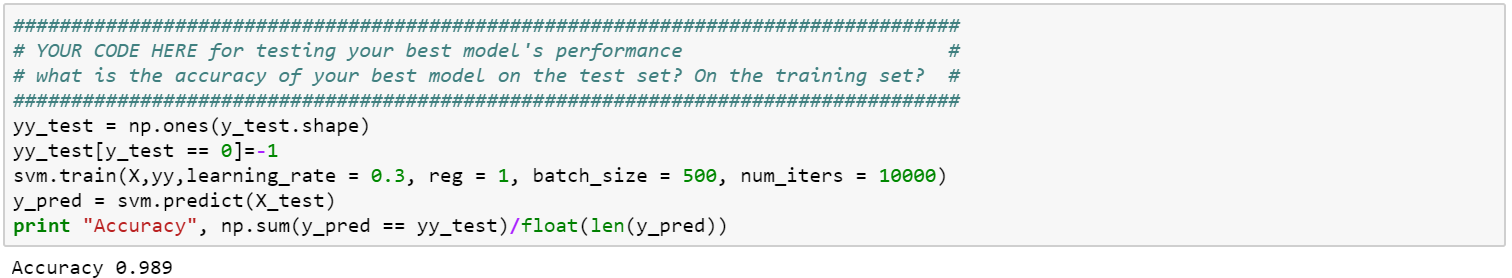
\includegraphics[width=12cm]{test.png}
	\caption{the test accuracy using the best hyperparameter}
	\label{fig:9}
\end{figure}
In order to speed up the process of selecting best parameters, we set the batch size to a smaller number. Using the best parameters we found, we achieve a test accuracy over 98.5%.
\begin{figure}[H]
	\centering
	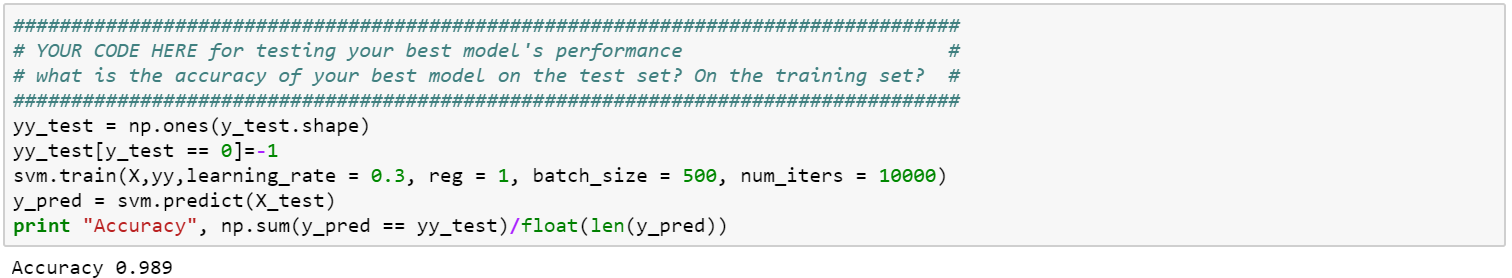
\includegraphics[width=12cm]{test.png}
	\caption{the test accuracy using the best hyperparameter}
	\label{fig:10}
\end{figure}
\begin{figure}[H]
	\centering
	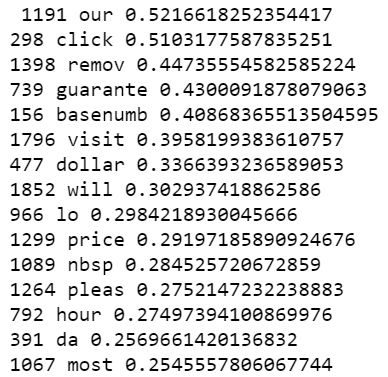
\includegraphics[width=8cm]{spam.png}
	\caption{the 15 words most indicative of spam}
	\label{fig:11}
\end{figure}
\begin{figure}[H]
	\centering
	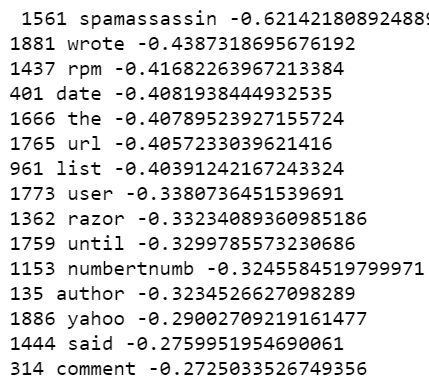
\includegraphics[width=8cm]{ham.png}
	\caption{the 15 words most indicative of ham}
	\label{fig:12}
\end{figure}
\subsection*{Part 4: Support vector machines for multi-class classification }

%% Problem 1
\begin{enumerate}
	\item It is possible that once in a while a dimension in the gradient check will not match exactly. What could such a discrepancy be caused by? Is it a reason for concern?
	\begin{soln}
		The discrepancy is caused by the non-differentiable part of the loss function. The loss function is non-differentiable in when $\theta^{(j)^{T}}x(i) - \theta^{y_i^{T}}x(i)+\Delta = 0$. \\
		It is not a reason for concern. The loss will not increase if gradient is computed this way. So it is not a reason for concern.  
	\end{soln}
	
	\item Loss history figure.
	\begin{soln}
		The loss changes with iteration times. The loss history plot is shown in Figure \ref{fig:lossHistory}.
		\begin{figure}[H]
			\centering
			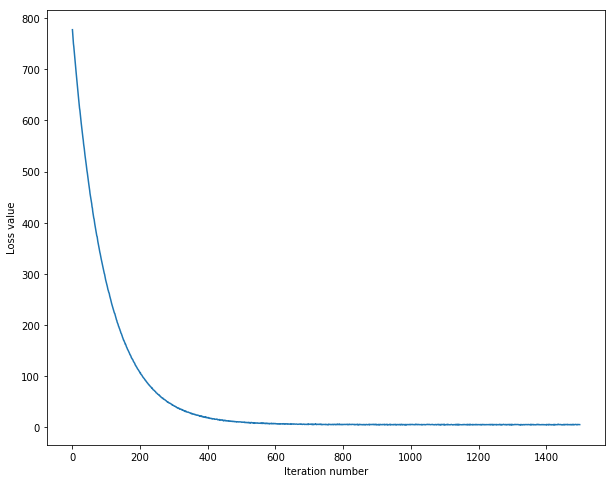
\includegraphics[width=8cm]{lossHistory.png}
			\caption{Loss History}
			\label{fig:lossHistory}
		\end{figure}
	\end{soln}
	
	
	\item Search for the best svm model.
	\begin{soln}
		Experiment with 4 learning rates and 4 regularization strengths. The result are:\\
		\textit{lr 1.000000e-08 reg 1.000000e+04 train accuracy: 0.230592 val accuracy: 0.249000\\
			lr 1.000000e-08 reg 5.000000e+04 train accuracy: 0.264000 val accuracy: 0.258000\\
			lr 1.000000e-08 reg 1.000000e+05 train accuracy: 0.301898 val accuracy: 0.321000\\
			lr 1.000000e-08 reg 5.000000e+05 train accuracy: 0.323796 val accuracy: 0.340000\\
			lr 5.000000e-08 reg 1.000000e+04 train accuracy: 0.315531 val accuracy: 0.323000\\
			lr 5.000000e-08 reg 5.000000e+04 train accuracy: 0.373837 val accuracy: 0.392000\\
			lr 5.000000e-08 reg 1.000000e+05 train accuracy: 0.360265 val accuracy: 0.374000\\
			lr 5.000000e-08 reg 5.000000e+05 train accuracy: 0.313184 val accuracy: 0.331000\\
			lr 1.000000e-07 reg 1.000000e+04 train accuracy: 0.372735 val accuracy: 0.376000\\
			lr 1.000000e-07 reg 5.000000e+04 train accuracy: 0.368714 val accuracy: 0.376000\\
			lr 1.000000e-07 reg 1.000000e+05 train accuracy: 0.354429 val accuracy: 0.357000\\
			lr 1.000000e-07 reg 5.000000e+05 train accuracy: 0.317000 val accuracy: 0.332000\\
			lr 5.000000e-07 reg 1.000000e+04 train accuracy: 0.369204 val accuracy: 0.369000\\
			lr 5.000000e-07 reg 5.000000e+04 train accuracy: 0.339816 val accuracy: 0.336000\\
			lr 5.000000e-07 reg 1.000000e+05 train accuracy: 0.291224 val accuracy: 0.292000\\
			lr 5.000000e-07 reg 5.000000e+05 train accuracy: 0.280633 val accuracy: 0.289000\\
			lr 1.000000e-06 reg 1.000000e+04 train accuracy: 0.362796 val accuracy: 0.375000\\
			lr 1.000000e-06 reg 5.000000e+04 train accuracy: 0.254204 val accuracy: 0.266000\\
			lr 1.000000e-06 reg 1.000000e+05 train accuracy: 0.265082 val accuracy: 0.277000\\
			lr 1.000000e-06 reg 5.000000e+05 train accuracy: 0.227735 val accuracy: 0.232000\\
			best validation accuracy achieved during cross-validation: 0.392000}
		
		Visualized the results and the results are shown in Figure \ref{fig:train_acc}.
		\begin{figure}[H]
			\centering
			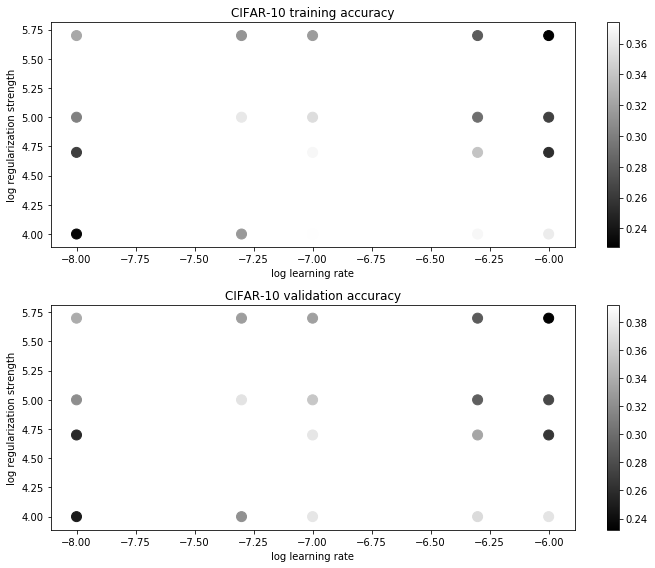
\includegraphics[width=8cm]{train_acc.png}
			\caption{Visualized Results for Parameter Selection}
			\label{fig:train_acc}
		\end{figure}
	\end{soln}
	
	
	\item Evaluate the test set accuracy on the best svm learned.
	\begin{soln}
		After searching for the best values of learning rate and regularization. We obtain the best svm model. The results on the test set is: \textit{linear SVM on raw pixels final test set accuracy: 0.368300.}\\
		The accuracy is similar to the accuracy of validation set. Visualization of the results is shown in Figure \ref{fig:multiSVM}.
		
		\begin{figure}[H]
			\centering
			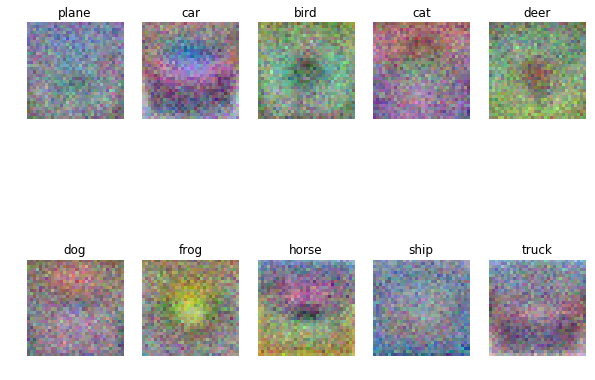
\includegraphics[width=8cm]{multiSVM_final.png}
			\caption{Visualized Results for Best SVM Multiclass Model}
			\label{fig:multiSVM}
		\end{figure}
		
	\end{soln}
	
	
	\item Comparing the performance of multi-class SVM and softmax regression. Which approach takes longer to train, which approach achieves higher performance? Compare the visualizations of the $\theta$ parameters learned by both methods - do you see any differences? Comment on hyper parameter selection for both methods.
	\begin{soln}
		\textbf{First compare the accuracy.}
		\begin{itemize}  
			\item Softmax on raw pixels final test set accuracy: 0.405100
			\item Linear SVM on raw pixels final test set accuracy: 0.368300.
		\end{itemize}
		The accuracy on Softmax and SVM are almost the same level. Softmax is slightly higher than linear SVM method.
		
		\textbf{Then compare the visualization of these two methods.}\\
		Figure \ref{fig:softmax} shows the results on softmax model.
		\begin{figure}[H]
			\centering
			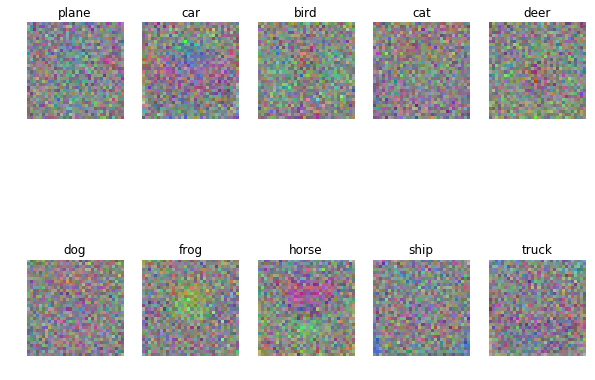
\includegraphics[width=8cm]{softmax_res.png}
			\caption{Visualized Results for Best Softmax Model}
			\label{fig:softmax}
		\end{figure}
		Figure \ref{fig:SVM} shows the results on SVM multiclass model.
		\begin{figure}[H]
			\centering
			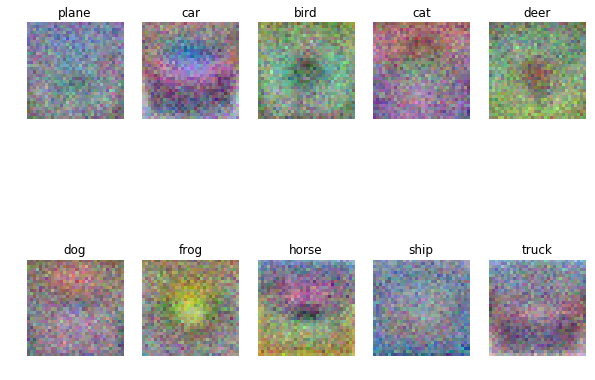
\includegraphics[width=8cm]{multiSVM_final.png}
			\caption{Visualized Results for Best SVM Multiclass Model}
			\label{fig:SVM}
		\end{figure}
		From the figure it seems the SVM model extracts a more "meaningful" features. Here "meaningful" means understandable for humans. The contour and edges are more clear in SVM model results.
		
		\textbf{Compare the time of these two methods.}
		\begin{itemize}
			\item Softmax vectorized loss: 2.352202e+00 computed in 0.483000s
			\item Linear SVM Vectorized loss: 9.293820e+00 computed in 0.016000s
		\end{itemize}
		In terms of time cost. Softmax takes a much longer time to train. The reason is that SVM learns a sparse kernel.
		
		
		
	\end{soln}
	
\end{enumerate}

\end{document}


